\chapter{Theory}
\section{Machine Learning}

Historically computers had to be programmed on a specific task using domain knowledge of humans. Machine learning challenges this traditional way of programming. Rather than trough extensive domain knowledge, machine learning algorithms are used to autonomously learn from data and information. 
\\
%https://www.forbes.com/sites/bernardmarr/2016/02/19/a-short-history-of-machine-learning-every-manager-should-read/#77bf286315e7

This intention is often represented by a 'learning' \emph{input-output function}. Assume there exists function, $f$, which represents a true behaviour or correlation. The task of any machine learning algorithm is thereby to find a \emph{hypothesis function} $h$ that resembles the behaviour of $f$ as closely as possible. A function $h$ is also called \emph{model}. Both $f$ and $h$ are function of a fixed length vector-valued input $X={x_1, x_2, ... , x_n}$ which has $n$ components. Those might be $n$ attributes of an observed object. An input $x$ is often referred to as a \emph{data point}. The components of a data point $x$ are the \emph{features} of $x$. 
The features of a data point span the \emph{feature space}. The feature space refers to the $n$-dimensional space in which the features of a data point are represented.
\\
The function $h$ can be thought of as a device that has $X$ as an input and $h(X)$ as an output. The hypothesis function, h, is selected based on a trainings set, $\Xi$, of $m$ input vector examples.
\\
There are two major settings in machine learning. 
\\
The first setting is \emph{unsupervised learning}. In this case the trainings set of vectors $\Xi$ doesn't provide information about the value $f(X)$ . The goal of the unsupervised learning algorithms usually is to partition the training set into subset, $\Xi$ \textsubscript{1}, $\Xi$ \textsubscript{2}, ..., $\Xi$ \textsubscript{r}. An example for unsupervised machine learning learning is \emph{clustering}, which finds clusters and discovers relationships in the data.
\\
The second is  \emph{supervised learning}, in which the values of $f$ for the samples in the training set $\Xi$ are known. The value of $f$ corresponding to a data point $x$ is also called the \emph{label} of $x$. A dataset with a label for every data point in it is referred to as a \emph{labelled} dataset. The assumption is that a hypothesis $h$ is a good guess for $f$ when $h(x_i)$ agrees with the values of $f(x_i)$ or the given labels for the majority of samples $x_i$ .
%classification application in pattern recognition 
% http://cs.du.edu/~mitchell/mario_books/Introduction_to_Machine_Learning_-_2e_-_Ethem_Alpaydin.pdf 6
\\
In supervised machine learning two main areas are distinguished, \emph{Regression} and \emph{Classification}. 
\\
In Regression the hypothesis $h$ has a continuous output. Regression could, for instance, be used to approximate a function for a stock price and predict a future stock price as a numerical value on a continuous range of possible prices.
\\
Classification has a categorical output. Classification could, for instance, be used to classify emails to either spam or no spam. It also finds application in patter recognition. % http://cs.du.edu/~mitchell/mario_books/Introduction_to_Machine_Learning_-_2e_-_Ethem_Alpaydin.pdf 6? 
The case of an classification task that has a need to classify data into two distinguished classes is called \emph{binary classification}. The alternative case is \emph{multiclass classification}, which aims to classify data points into one of multiple different classes.

%classification, inpu, representation, hypotesis, generalization:
% http://cs.du.edu/~mitchell/mario_books/Introduction_to_Machine_Learning_-_2e_-_Ethem_Alpaydin.pdf 21

\section{Evaluation of Classifiers}
\begin{itemize}
\item{f-score}
fscore , precision, recall
% http://delivery.acm.org/10.1145/320000/312647/p42-yang.pdf?ip=134.155.178.109&id=312647&acc=ACTIVE%20SERVICE&key=2BA2C432AB83DA15%2E33B98ACB330D6FA0%2E4D4702B0C3E38B35%2E4D4702B0C3E38B35&CFID=976370719&CFTOKEN=43508633&__acm__=1503605339_b0f297be35db501d0410685c60e0b4b6
(2 oben rechts)
\item{Cross validation}
% https://wiki.eecs.yorku.ca/course_archive/2014-15/F/4412/_media/ensemble_data_mining.pdf 26 (44)

especially k-fold validation: 
is non exhaustive

% http://ai.stanford.edu/people/nilsson/MLBOOK.pdf  82

\end{itemize}
\section{Algorithms}
\begin{itemize}
\item{hyper-parameters}
% http://jmlr.csail.mit.edu/papers/volume13/bergstra12a/bergstra12a.pdf 2
\end{itemize}
\subsection{Linear support vector classifier}
In this chapter the support vector classifier will be introduced. The method was developed in the 1990’s and is often used as one of the best performing 'out of the box' classifiers. The support vector classifier is a extension of a maximal margin classifier. First  the concept of classification using a hyperplane and with a maximal margin classifier will be explained. Then the extension to a support vector classifier will be shown.

\subsubsection{Hyperplane classification}
The goal of the maximal margin classifier is to classify data by finding a hyperplane that optimally separates two classes in a dataset. Data points are either in class $y=f(x)=-1)$ or $y=f(x)=1)$. 
\\
A hyperplane is a flat affine subspace of dimension $p-1$, where p is the number of dimensions the hyperplane is in. In the case of a maximal margin classifier the number of dimensions which a hyperplane will be constructed in is the number dimension of the feature space. This stems from the intention to separate data points which have a feature vector of $p$ dimensions. Accordingly a hyperplane is defined by
\begin{equation} \label{eq:1}
\beta_0 + \beta_1 X_1 + ... + \beta_p X_p = 0
\end{equation}
for a feature space of dimension p. It can be said that $\beta_0$  to $\beta_p$ 'define' the hyperplane.
If a point $X=(x_1,x_2,...,x_p)$ lies on the hyperplane, the point features $x_1$ to $x_p$ would satisfy the equation \ref{eq:1}.
\\
If this doesn't hold true but
\begin{equation} \label{eq:2}
\beta _0 + \beta _1 X_1 + ... + \beta_p X_p > 0
\end{equation}
is true, the point $X$ lies on the one side of the plane, whereas if 
\begin{equation} \label{eq:3}
\beta_0 + \beta_1 X_1 + ... + \beta_p X_p < 0
\end{equation}
is true, the the point $X$ lies on the other side. 
\\
If a hyperplane is defined in a way that the data points of on class lay on the one side of the hyperplane and the data points of the other class on the other side, any given data point can be classified accordingly as either one or the other class according to equations \ref{eq:2} and \ref{eq:3}.
\\
The \emph{magnitude} of $h(X)$ can be used to derive a confidence score for the classification. A higher magnitude of $h(X)$, which can be interpreted as distance to the plane, corresponds to a higher confidence in the classification.


\subsubsection{Maximal margin classifier}

If a class separating hyperplane exist there exists an infinite number of such hyperplanes separating the classes (a hyperplane can always be moved or varied slightly while still remaining class separating). The question arises which hyperplane should be used. 
\\
A maximal margin classifier uses the hyperplane, where the distance to the next data point  is the biggest under all possibilities. The distance to the next data point is called the \emph{margin}. A hyperplane that has the biggest possible margin is a \emph{maximal margin hyperplane}. Data points where the distance to the maximal margin hyperplane is equal to the margin are the \emph{support vectors} as seen in figure \ref{fig:mmh}. The maximal margin hyperplane depends on the support vectors because moving or removing the support vectors would change the hyperplane. Moreover the vectors that are further away from the hyperplane than the support vectors don't contribute to definition of the hyperplane. This allows the hyperplane to be soly defined by the support vectors.\\

\begin{figure}[h]
\centering
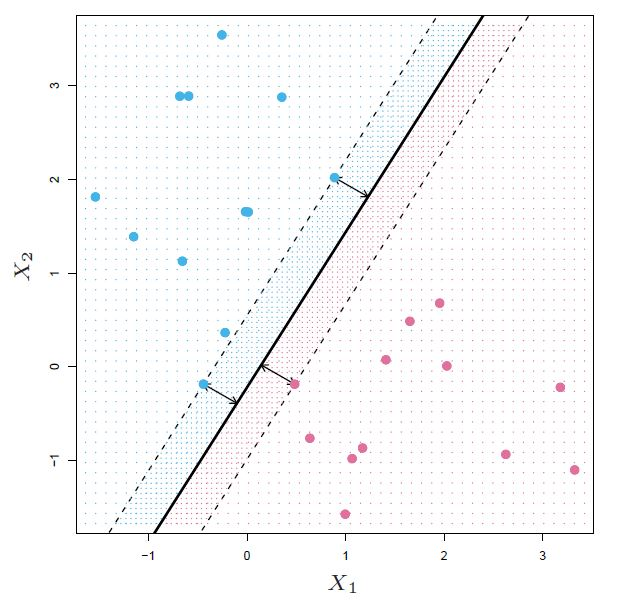
\includegraphics[width=0.7\textwidth]{PE4/svm.JPG}
\caption{Maximal margin hyperplane separating two classes of data points with the margin borders visualized by dotted lines}
\label{fig:mmh}
\end{figure}

To find a maximal margin hyperplane the parameters of the hyperplane have to be set in a way that maximises the size of the margin $M$ and
\begin{equation} \label{eq:7}
y_i(\beta_0+beta_1 x_i1 +\beta_2 x_i2 + ... +\beta_p x_ip) \leq M   \forall i=1,...,n
\end{equation}
holds.
$y_i$ is the true class of the $i$th data point. If all data points are classified correctly, which is the goal, the left side of the equation \ref{eq:7} is always positive. This is because either both $y_i$ and $f(X_i)$ are negative or both are positive. The right side of the equation makes sure that every data point has a minimal distance of M to the hyperplane.

The maximal margin classifier has some faults that have to be considered. Because the data points are of a class are strictly separated by a hyperplane of a linear form from the other class, it is not possible to find a hyperplane if the classes are not linear separable.  Furthermore even when the classes are linear separable the hyperplane pound might be forced in a unfavourable spot by only one single data point that doesn't represent most of the other data points of the same class. The extension to a support vector classifier solves those problems.

\subsubsection{Support vector classifier}

To solve the above mentioned faults the \emph{support vector classifier}, also called \emph{soft margin classifier}, allows some data points of the training data to be not on the correct side of the margin or the hyperplane. 
\\
To find a hyperplane for a support vector classifier the parameters of the hyperplane have to be set in a way that maximises the size of the margin $M$ and the equations 
\begin{equation} \label{eq:8}
y_i(\beta_0+beta_1 x_i1 +\beta_2 x_i2 + ... +\beta_p x_ip) \leq M(1- \epsilon_i ) \forall i=1,...,n
\end{equation}

\begin{equation} \label{eq:9}
\epsilon_i >= 0, \sum_i=1^n \epsilon_i \leq	 C
\end{equation}

both hold.\\
The concept is similar to the one seen in equation \ref{eq:7}. Differentiating here are the \emph{slack variables} $\epsilon_1, ..., \epsilon_n$. $\epsilon_i$ indicates where the $i$th data point is located relative to the hyperplane and it's margin. If the $i$th data point is on the correct side of the margin $\epsilon_i=0$. If the $i$th data point is on the correct side of the hyperplane but on the wrong side of the margin it \emph{violates} the margin and $\epsilon_i=0$. If the $i$th data point is on the wrong side of the hyperplane then $\epsilon_i=0$.  \\
C is a tuning parameter that limits the total sum of $e_i$s.\\
A bigger C allows more datapoints to violate the margin or be on the wrong side of the hyperplane. \\
This way a hyperplane can be found even when the classes are not strictly linearly separable and isolated outlier data points that would  distort the resulting hyperplane can be mostly ignored.\\


With a support vector classifier it's now possible to create a model $h$ that can be trained on data with non linear separable classes. The model takes a data point and classifies it to either one class ($h(x)<0$) or the other class ($h(x)>0$). The magnitude $|h(x)|$ can be interpreted as confidence score of the classification.
 
%An introduction to statistical learning

\subsection{Logistic regression}

The goal of logistic regression is to create a classifier which predicts the probability for a given data point $X$ to belong to a certain class $c$. This probability	 of a class $c$ under the condition of $X$ can be written as
\begin{equation} \label{eq:4}
p(c|X) \in [0,1]
\end{equation}
The model $h(X)=p(c=1|X)$ gives the probability of a data point $X$ being of the class 1.
\\

Logistic regression is based on a linear regression. Linear regression models a linear function. It tries to choose the function parameters $\beta_0, ..., \beta_p$ in a way  that the function approximately goes through every data point in the training data it was derived from. \ref{eq:5}. 
\begin{equation} \label{eq:5}
y=\beta_0 + \beta_1 x_1 + \beta_2 x_2 + ... + + \beta_n x_n
\end{equation}
How this can be done exactly is out scope for this paper. The focus is on the classification algorithm logistic regression.\\
Logistic regression tries to create a model predicting probability, hence a value $p \in [0,1]$ . \\
The \emph{standard logistic function}, as seen in \ref{eq:10}, has the property of mapping an input to a range of 0 to 1. The codomain of the standart logistic function is 0 to 1.
\begin{equation} \label{eq:10}
f(x)=\frac{1}{1+e^-x}=\frac{e^x}{1+e^x}
\end{equation}
Utilizing the linear regression in equation \ref{eq:5} the output is now transformed with the standart logistic function:

\begin{equation} \label{eq:10}
h(x)=\frac{e^{\beta_0 + \beta_1 x_1 + \beta_2 x_2 + ... + \beta_n x_n}}{1+e^{\beta_0 + \beta_1 x_1 + \beta_2 x_2 + ... + + \beta_n x_n}}
\end{equation}

The function parameters $\beta_1$ to  $\beta_n$ are estimated based on the given data points.  \\
This way logistic regression creates a model which predicts the probability of a data point being in a certain class.


% https://www.jstor.org/stable/pdf/2983890.pdf?refreqid=excelsior:3ac2d6a000fa78f731ab46b8659528c0
D. R. Cox, The Regression Analysis of Binary Sequences 1958
\subsection{Decision tree}
% https://wiki.eecs.yorku.ca/course_archive/2014-15/F/4412/_media/ensemble_data_mining.pdf 54 (somewhere)
\subsection{Random forest}
% https://wiki.eecs.yorku.ca/course_archive/2014-15/F/4412/_media/ensemble_data_mining.pdf 54 (72)
\subsection{Gradient-boosted trees}
% https://wiki.eecs.yorku.ca/course_archive/2014-15/F/4412/_media/ensemble_data_mining.pdf 54 (somewhere)
\subsection{Naive Bayes}
% http://researchweb.watson.ibm.com/people/r/rish/papers/RC22230.pdf (IBM ressource)
info PDF in quellen